\documentclass[a4paper]{article}

%% Language and font encodings
\usepackage[english]{babel}
\usepackage[utf8x]{inputenc}
\usepackage[T1]{fontenc}

%% Sets page size and margins
\usepackage[a4paper,top=3cm,bottom=2cm,left=3cm,right=3cm,marginparwidth=2cm]{geometry}

%% Useful packages
\usepackage{algorithm}
\usepackage{amsfonts}
\usepackage{amsmath}
\usepackage{amssymb}
\usepackage{amsthm}
\usepackage{bbm}
\usepackage[colorinlistoftodos]{todonotes}
% \usepackage[colorlinks=true, allcolors=blue]{hyperref}
\usepackage{enumerate}
\usepackage{float}
\usepackage{graphicx}
\usepackage{mathrsfs}
\usepackage{subcaption}
\usepackage{tikz}
\usepackage{tikzscale}
\usetikzlibrary{shapes.geometric, arrows}
\tikzset{
    vertex/.style={circle,draw,minimum size=1.5em},
    edge/.style={->,> = latex'}
}
\tikzstyle{triger} = [circle, minimum width=2cm, minimum height=1cm, text centered, draw=black]
\tikzstyle{process} = [rectangle, minimum width=1cm, minimum height=1cm, text centered, draw=black]
\tikzstyle{decision} = [diamond, minimum width=2cm, minimum height=1cm, text centered, draw=black]
\tikzstyle{block} = [rectangle, minimum width=3cm, minimum height=3cm, text centered, draw=black]
\tikzstyle{arrow} = [thick,->,>=stealth]

\title{HW1}
\author{Kevin Chang}

\newtheorem{definition}{Definition}
\newtheorem{problem}{Problem}
\newtheorem{property}{Property}[section]
\newtheorem{theorem}{Theorem}[section]
\newtheorem{suspect}{Suspect}[section]
\newtheorem{example}{Example}
\newtheorem{lemma}[theorem]{Lemma}

\graphicspath{ {./images/} }

\begin{document}
\maketitle

\paragraph{Terminology}
\begin{itemize}
    \item System state $Y$: an unknown random variable.
    \item Measurement $X$: an observed random variable statistically related to $Y$.
    \item Estimator $\hat{Y}(X)$: a random variable defined as a function of $X$.
    \item Probability:
    \begin{itemize}
        \item Prior: $P[Y]$
        \item Posterior: $P[Y \mid X]$
        \item Likelihood: $P[X \mid Y]$
    \end{itemize}
    \item Objective (Risk):  
    \[
        R[\hat{Y}] = \mathbb{E}\big[\mathit{loss}(\hat{Y}(X), Y)\big]
    \]
    
    \item Optimal Estimator (Posterior form):  
        $$\hat{Y}(x) = \mathbbm{1}\!\left\{ 
        P[Y = 1 \mid X = x ] \;\geq\; 
        \frac{\mathit{loss}(1,0) - \mathit{loss}(0,0)}{\mathit{loss}(0,1) - \mathit{loss}(1,1)} 
        \, P[Y = 0 \mid X = x ] \right\}$$

    \begin{itemize}
        \item Proof:  
            $$\mathbb{E}[\mathit{loss}(\hat{Y}(X), Y)] = \int_{-\infty}^\infty \mathbb{E}[\mathit{loss}(\hat{Y}(X), Y) \mid X=x] f_X(x)\, dx$$
            {\tiny$$= \int_{-\infty}^\infty \Big(
            \mathbb{E}[\mathit{loss}(\hat{Y}(X), 1) \mid X=x] \, P[Y=1 \mid X=x]
            + \mathbb{E}[\mathit{loss}(\hat{Y}(X), 0) \mid X=x] \, P[Y=0 \mid X=x]
        \Big) f_X(x)\, dx$$}
        \item Thus, $\hat{Y}(x)$ is chosen according to the label (0 or 1) that minimizes the conditional expected loss.
    \end{itemize}

    \item Optimal Estimator (Likelihood ratio form):  
    \[
    \hat{Y}(x) = \mathbbm{1}\!\left\{ 
        \frac{p(x \mid Y=1)}{p(x \mid Y=0)} 
        \;\geq\;
        \frac{p_0 \, \big(\mathit{loss}(1,0) - \mathit{loss}(0,0)\big)}{p_1 \, \big(\mathit{loss}(0,1) - \mathit{loss}(1,1)\big)}
    \right\}
    \]

    \begin{itemize}
        \item Proof by rearrangement of the posterior condition.
        \item This corresponds to a \emph{likelihood ratio test}.
    \end{itemize}
\end{itemize}

\paragraph{Types of errors and successes}
\begin{itemize}
    \item True Positive Rate: $P[\hat{Y} = 1| Y=1]$
    \item False Negative Rate: $P[\hat{Y} = 0| Y=1]$
    \item False Positive Rate: $P[\hat{Y} = 1| Y=0]$
    \item True Negative Rate: $P[\hat{Y} = 0| Y=0]$
    \item Precision: $P[Y = 1| \hat{Y}=1]$
\end{itemize}

\paragraph{Receiver Operating Characteristic(ROC) curve}

\begin{itemize}
    \item Example
    \begin{figure} [H]
        \centering
        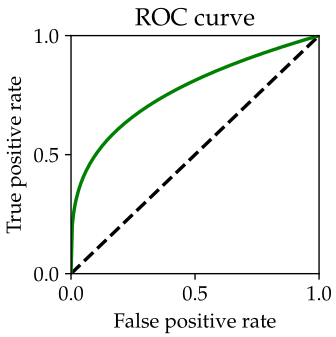
\includegraphics[width=0.5\linewidth]{image/roc.png}
        \caption{The ROC curve is plotted in the FPR–TPR plane.}
    \end{figure}
    \item Lemma 2 (Neyman–Pearson Lemma)
Suppose the likelihood functions $p(x \mid y)$ are continuous. Then the optimal probabilistic predictor that maximizes TPR subject to an upper bound on FPR is a deterministic likelihood ratio test.
    \item Properties
        \begin{itemize}
            \item always passes through $(0,0)$ and $(1,1)$,
            \item must lie above the main diagonal,
            \item is concave.
        \end{itemize}
\end{itemize}

\paragraph{Fairness}
\begin{itemize}
    \item Key statistical measures include:
        \begin{itemize}
            \item \textbf{Acceptance rate:} $\Pr[\hat{Y} = 1]$
            \item \textbf{Error rates:} $\Pr[\hat{Y} = 0 \mid Y = 1],\; \Pr[\hat{Y} = 1 \mid Y = 0]$
            \item \textbf{Conditional outcome frequency:} $\Pr[Y = 1 \mid R = r]$
        \end{itemize}

    \item Standard fairness criteria are:
        \begin{itemize}
            \item \textbf{Independence:} $R \perp A$ \quad (equal acceptance rates across groups)
            \item \textbf{Separation:} $R \perp A \mid Y$ \quad (equal error rates across groups)
            \item \textbf{Sufficiency:} $Y \perp A \mid R$ \quad (equal outcome frequencies given $R$)
        \end{itemize}
    \item It is well known that any two criteria are mutually exclusive in general, except in degenerate cases; thus enforcing one typically precludes the others.
\end{itemize}

\section{Supervised Learning}
Let $S = \{(x_1, y_1), \ldots, (x_n, y_n)\}$ denote a labeled dataset with $x_i \in \mathcal{X}$ and $y_i \in \mathcal{Y}$.  
For a predictor $f: \mathcal{X} \to \mathcal{Y}$, the \emph{empirical risk} is
\[
    R_S[f] = \frac{1}{n} \sum_{i=1}^n \mathit{loss}\big(f(x_i), y_i\big),
\]

Three fundamental questions arise:
\begin{itemize}
    \item \textbf{Representation:} Which function class $\mathcal{F}$ should we select?
    \item \textbf{Optimization:} How can the corresponding learning problem be solved efficiently?
    \item \textbf{Generalization:} How well does the predictor extend from training data to unseen samples?
\end{itemize}

\paragraph{Perceptron Algorithm}
The perceptron iteratively updates a weight vector $w \in \mathbb{R}^d$:
\begin{itemize}
    \item Initialize $w^{(0)} = 0$.
    \item For $t = 0, 1, 2, \ldots$:
    \begin{itemize}
        \item Select $i \in \{1, \ldots, n\}$ uniformly at random.
        \item If $y_i \langle w^{(t)}, x_i \rangle < 1$, set
        \[
        w^{(t+1)} = w^{(t)} + y_i x_i,
        \]
        else $w^{(t+1)} = w^{(t)}$.
    \end{itemize}
\end{itemize}

\paragraph{Connection to Empirical Risk Minimization}
The perceptron update can be viewed as stochastic gradient descent (SGD) on Hinge loss:  
    $$\min_w \frac{1}{n} \sum_{i=1}^n \ell_{\mathrm{hinge}}(y_i, \langle w, x_i \rangle) + \|w\|_2^2.$$
\begin{itemize}
    \item \textbf{Hinge loss:} 
    \[
    \ell_{\mathrm{hinge}}(y, \hat{y}) = \max\{1 - y\hat{y}, 0\}, \quad 
    \]
    \item \textbf{Squared loss:} 
    \[
    \ell_{\mathrm{sq}}(y, \hat{y}) = \tfrac{1}{2}(y - \hat{y})^2, 
    \]
    \item \textbf{Logistic loss:} 
    \[
    \ell_{\mathrm{log}}(y, \hat{y}) = 
    \begin{cases}
        -\log(\sigma(\hat{y})), & y=1, \\
        -\log(1-\sigma(\hat{y})), & y=-1,
    \end{cases}
    \]
    where $\sigma(z) = \tfrac{1}{1+e^{-z}}$ is the sigmoid.
\end{itemize}

\paragraph{Margin Analysis}
\begin{itemize}
    \item For $w \in \mathbb{R}^d$, define the \emph{margin} on dataset $S$ as
\[
\gamma(S, w) = \min_{1 \leq i \leq n} \frac{| \langle x_i, w \rangle |}{\|w\|}, 
\qquad \gamma(S) = \max_w \gamma(S, w).
\]
    \item Let $D(S) = \max_{1 \leq i \leq n} \|x_i\|$.  
    \item Theorem: If $S$ is linearly separable, the perceptron algorithm makes at most $\frac{\big(2 + D(S)^2\big)}{\,\gamma(S)^2}$ margin mistakes.
    \item \emph{Proof sketch.} Expanding the update yields
\[
\|w^{(t+1)}\|^2 = \|w^{(t)} + y_i x_i\|^2 
= \|w^{(t)}\|^2 + 2y_i \langle w^{(t)}, x_i \rangle + \|x_i\|^2
\le \|w^{(t)}\|^2 + 2 + D(S)^2.
\]
Meanwhile, progress in the margin direction ensures
\[
\langle w^\ast, w^{(t+1)} - w^{(t)} \rangle \ge \gamma(S),
\]
for an optimal separator $w^\ast$, leading to the stated bound.

\end{itemize}

\paragraph{Generalization Bound}
Let $S_n$ be $n$ i.i.d.\ samples from a distribution $\mathcal{D}$ admitting a perfect linear separator.  
Let $w(S_n)$ denote the perceptron’s output after convergence on $S_n$, and let $(X,Y) \sim \mathcal{D}$ be independent of $S_n$.  
Then
\[
    P\!\left[Y w(S_n)^T X < 1 \right] \leq \mathbb{E}[\frac{2 + D(S_{n+1})^2}{(n+1)\,\gamma(S_{n+1})^2}],
\]
where $D(S_{n+1})$ and $\gamma(S_{n+1})$ are defined analogously on $S_{n+1} = S_n \cup \{(X,Y)\}$.


\section{Representation}
\begin{itemize}
    \item \textbf{Lifting functions $\Phi(x)$:} Transform a given set of features into a more expressive feature space.
    \item \textbf{Common strategies:}
    \begin{itemize}
        \item \textbf{Template matching:} For example, $x_0 = \max\{v^\top x, 0\}$, which can be interpreted as a sliding window that activates when a feature satisfies certain conditions.
        \item \textbf{Polynomial features:} In $d$ dimensions with maximum degree $p$, the number of monomial coefficients is $\binom{d+p}{p}$.
    \end{itemize}
    \item \textbf{Dimensionality:} How high must the lifted dimension be?  

    To gain intuition, stack $n$ data points $x_1, \ldots, x_n \in \mathbb{R}^d$ into a matrix $X \in \mathbb{R}^{n \times d}$, where each row corresponds to a sample. Predictions over the dataset can then be expressed as
    \[
    \hat{y} = Xw.
    \]
    If the $x_i$ are linearly independent and $d \geq n$, then any prediction vector $y$ can be realized by an appropriate weight vector $w$. Thus, feature design often aims to lift data into sufficiently high-dimensional spaces so that the feature matrix $X$ has linearly independent columns, enabling greater expressivity.

    \item \textbf{Kernels}
        \begin{itemize}
            \item Given a lifting functoin $\Phi$, the kernel function is
        \[
        k(x,z) := \Phi(x)^\top \Phi(z),
        \]
        which ensures that for any $x_1,\dots,x_n$, the Gram matrix $K$ with entries $K_{ij}=k(x_i,x_j)$ is positive semidefinite.

            \item A function $f$ can be expressed as
        \[
            f(x) = w^\top \Phi(x) = \sum_{1 \leq i \leq n} \alpha_i \, k(x_i, x).
        \]
            \item Moreover, if $k_1$ and $k_2$ are kernels, then both $k_1 k_2$ and $k_1 + k_2$ are valid kernels.
        \end{itemize}
\end{itemize}

\section{Optimization}
\begin{itemize}
    \item \textbf{Gradient Descent.}  
        \begin{itemize}
            \item \textit{Procedure.}
                \begin{itemize}
                    \item Minimize the empirical loss  
                    \[
                        \phi(w) = \frac{1}{n} \sum_{i=1}^n \mathcal{L}(f(x_i, w), y_i).
                    \]
                    \item Initialize $w_0 \in \mathbb{R}^d$.
                    \item For $t = 0, 1, 2, \dots$:  
                    \[
                        w_{t+1} = w_t - \alpha_t \frac{1}{n} \sum_{i=1}^n \nabla \mathcal{L}(f(x_i, w), y_i), \quad \alpha_t > 0.
                    \]
                \end{itemize}

            \item \textit{Theorem.}
                \begin{itemize}
                    \item A vector $v$ is a descent direction for $\phi$ at $w_0$ if  
                    \[
                        \phi(w_0 + t v) < \phi(w_0) \quad \text{for some } t > 0.
                    \]  
                    \item A point $w^\ast$ is a local minimizer only if $\nabla \phi(w^\ast) = 0$.  
                    \item If $\phi : \mathbb{R}^d \to \mathbb{R}$ is differentiable and convex, then  
                    \[
                        w^\ast \text{ is a global minimizer of } \phi \iff \nabla \phi(w^\ast) = 0.
                    \]
                \end{itemize}
        \end{itemize}
    \item \textbf{Stochastic Gradient Descent (SGD).}  
        \begin{itemize}
            \item \textit{Procedure.}
                \begin{itemize}
                    \item Minimize the empirical loss  
                    \[
                        \phi(w) = \frac{1}{n} \sum_{i=1}^n \mathcal{L}(f(x_i, w), y_i).
                    \]
                    \item Initialize $w_0 \in \mathbb{R}^d$.
                    \item For $t = 0, 1, 2, \dots$, sample $i \in \{1,\dots,n\}$ uniformly at random and update  
                    \[
                        w_{t+1} = w_t - \alpha_t \nabla_w \mathcal{L}(f(x_i, w_t), y_i), 
                        \quad \alpha_t > 0.
                    \]
                \end{itemize}

            \item \textit{Remark.}  
            SGD reduces to the perceptron algorithm when applied with the hinge-type loss  
            \[
                \ell(y, \hat{y}) = \max(-y \hat{y}, 0),
            \]  
            using a linear predictor $f(x, w) = w^\top x$.
            % \item \textit{Analysis}
            %     $g_t(w_t, \eta_t) = $ sample value $\nabla_w \mathcal{L}(f(x_i, w_t), y_i)$
            %
            % $||g(w, \eta)||\leq B$
            % $\sum_{s=0}^t \alpha_s \mathcal{L}(f(x_s, w_s), y_s) - \sum_{s=0}^t \alpha_s \mathcal{L}(f(x_s, w_*), y_s) \leq \frac{||w_0 - w_*||^2 + B^2 \sum_{t=0}^T \alpha_t^2}{2 \sum_{t=0}^T \alpha_t^2}

            \item \textit{Analysis.}  
                \begin{itemize}
                    \item Assume SGD update rule is given by
                        $$w_{t+1} = w_t - \alpha_t g_t(w_t; \eta_t),$$
            ,where \( g_t(w_t, \eta_t) = \nabla_w \mathcal{L}(f(x_t, w_t), y_t) \) is a stochastic gradient computed from a sample \(\eta_t = (x_t, y_t)\).
                    \item Assume the gradient is bounded:
                        $$\| g_t(w_t; \eta_t) \| \le B, \quad \forall t.$$
                    \item We expand the squared norm of the distance to the optimum \( w_* \):
                        $$ \| w_{t+1} - w_* \|^2
            = \| w_t - w_* \|^2
            - 2 \alpha_t \langle g_t(w_t; \eta_t), w_t - w_* \rangle
            + \alpha_t^2 \| g_t(w_t; \eta_t) \|^2.$$
                    \item Taking expectations and using the law of iterated expectation gives
                        $$\mathbb{E}[\langle g_t(w_t; \eta_t), w_t - w_* \rangle] = \mathbb{E}[\langle \nabla \mathcal{L}(w_t), w_t - w_* \rangle].$$
                    \item Summing from \(t = 0\) to \(T-1\) and rearranging terms yields
                        $$\sum_{t=0}^{T-1} \alpha_t \mathbb{E}[\langle \nabla \mathcal{L}(w_t), w_t - w_* \rangle]
            \le \frac{1}{2}\|w_0 - w_*\|^2 + \frac{B^2}{2}\sum_{t=0}^{T-1}\alpha_t^2.
            $$
                    \item By convexity of \(\mathcal{L}\),
                        $$\mathcal{L}(w_t) - \mathcal{L}(w_*) \le \langle \nabla \mathcal{L}(w_t), w_t - w_* \rangle.$$
                    \item Hence,
                        $$\sum_{t=0}^{T-1} \alpha_t \mathbb{E}[\mathcal{L}(w_t) - \mathcal{L}(w_*)]
            \le \frac{\|w_0 - w_*\|^2}{2} + \frac{B^2}{2}\sum_{t=0}^{T-1}\alpha_t^2.$$


                    \item Defining the weighted average iterate
                        $$\tilde{w}_T = \frac{\sum_{t=0}^{T-1}\alpha_t w_t}{\sum_{t=0}^{T-1}\alpha_t},$$
                    \item and applying convexity again, we obtain the standard SGD convergence bound:
                        $$ \mathbb{E}[\mathcal{L}(\tilde{w}_T) - \mathcal{L}(w_*)] \le
                \frac{\|w_0 - w_*\|^2 + B^2 \sum_{t=0}^{T-1}\alpha_t^2} {2 \sum_{t=0}^{T-1}\alpha_t}.$$
                \end{itemize}

        \end{itemize}
\end{itemize}

\section{Generalization}
\begin{itemize}
    \item The goal is to bound the difference between the \emph{empirical risk} $R_S[f]$ (measured on a sample) and the \emph{true risk} $R[f]$ (expected loss under the underlying distribution).

    \item \textbf{Hoeffding’s Inequality.}
    For independent random variables $Z_1, \dots, Z_n$ bounded in $[a_i, b_i]$,
    \[
    P[\bar{Z} - \mathbb{E}[\bar{Z}] \ge t]
    \le 
    \exp\!\left(-\frac{2n^2 t^2}{\sum_{i=1}^n (b_i - a_i)^2}\right),
    \quad
    \bar{Z} = \tfrac{1}{n}\sum_{i=1}^n Z_i.
    \]
    If the loss $\mathcal{L}$ is bounded in $[0,1]$, then for any $f$,
    \[
    P[R_S[f] > R[f] + t] \le e^{-2nt^2}.
    \]

    \item \textbf{Finite Hypothesis Class.}
    Applying the union bound to a finite hypothesis set $\mathcal{F}$ yields, with probability at least $1 - \delta$,
    \[
    |R_S[f] - R[f]|
    \le
    \sqrt{\frac{\ln|\mathcal{F}| + \ln(1/\delta)}{2n}},
    \quad
    \forall f \in \mathcal{F},
    \]
    where $\ln|\mathcal{F}|$ measures the \emph{complexity} of the model family. 
    The generalization gap thus scales as
    $\mathcal{O}\!\left(\sqrt{\tfrac{\text{complexity}(\mathcal{F})}{n}}\right)$.

    \item \textbf{Confidence Interval.}
        \begin{itemize}
            \item A confidence interval asserts that, with probability at least \(1 - \delta\), a random variable \(Z\) lies within a (possibly random) set \(A\); that is,
            \[
            \Pr[\, Z \in A \,] \geq 1 - \delta,
            \]
            where both \(Z\) and \(A\) may depend on random quantities.
        \end{itemize}

    \item \textbf{PAC Learning.}
        \begin{itemize}
            \item A learning algorithm is said to be \((\epsilon, \delta)\)-PAC if, with probability at least \(1 - \delta\) over the sampling of the training set \(S\), the expected loss satisfies
            \[
            \mathbb{E}[\mathrm{loss}(f_S(x), y) \mid S] \leq \epsilon.
            \]
        \end{itemize}
\end{itemize}



\end{document}

